\documentclass[border=8pt]{standalone}
\usepackage[T1]{fontenc}\usepackage[utf8]{inputenc}
\usepackage{helvet}\renewcommand{\familydefault}{\sfdefault}
\usepackage{tikz,xcolor}
\usetikzlibrary{arrows.meta,positioning,shapes.geometric,shapes.multipart,calc,fit,backgrounds,decorations.markings}
\definecolor{ink}{HTML}{1E1B16}\definecolor{paper}{HTML}{FBF8F2}\definecolor{clay}{HTML}{B5482A}\definecolor{soft}{HTML}{F1E9DA}\definecolor{pine}{HTML}{24402F}
\tikzset{
  every node/.style={font=\small,text=ink},
  >=Stealth, line/.style={draw=ink,line width=0.8pt},
  cls/.style={rectangle split,rectangle split parts=3,draw=ink,line width=0.8pt,fill=soft,align=left,inner xsep=6pt,inner ysep=4pt,
              rectangle split part align={center,left,left},minimum width=3.0cm},
  cls2/.style={rectangle split,rectangle split parts=2,draw=ink,line width=0.8pt,fill=soft,align=left,inner xsep=6pt,inner ysep=4pt,
              rectangle split part align={center,left},minimum width=3.0cm},
  box/.style={rectangle,draw=ink,line width=0.8pt,fill=soft,align=center,inner sep=5pt,minimum height=0.8cm},
  state/.style={rectangle,rounded corners=8pt,draw=ink,line width=0.8pt,fill=soft,align=center,inner sep=6pt,minimum width=2.2cm,minimum height=0.9cm},
  act/.style={rectangle,rounded corners=10pt,draw=ink,line width=0.8pt,fill=soft,align=center,inner sep=5pt,minimum width=2.4cm,minimum height=0.8cm},
  dec/.style={diamond,draw=ink,line width=0.8pt,fill=soft,inner sep=1pt,minimum width=0.9cm,minimum height=0.9cm},
  uc/.style={ellipse,draw=ink,line width=0.8pt,fill=soft,align=center,inner sep=3pt,minimum width=3.2cm,minimum height=1.0cm},
  note/.style={rectangle,draw=ink,line width=0.6pt,fill=yellow!12,align=left,inner sep=4pt,font=\footnotesize},
  lab/.style={font=\footnotesize,fill=paper,inner sep=1.5pt},
  err/.style={},
}
\newcommand{\actor}[3]{% x,y,label
  \draw[line width=0.8pt] (#1,#2+0.55) circle (0.17);
  \draw[line width=0.8pt] (#1,#2+0.38)--(#1,#2-0.15) (#1-0.3,#2+0.22)--(#1+0.3,#2+0.22) (#1,#2-0.15)--(#1-0.25,#2-0.6) (#1,#2-0.15)--(#1+0.25,#2-0.6);
  \node[font=\small] at (#1,#2-0.9) {#3};}
\begin{document}
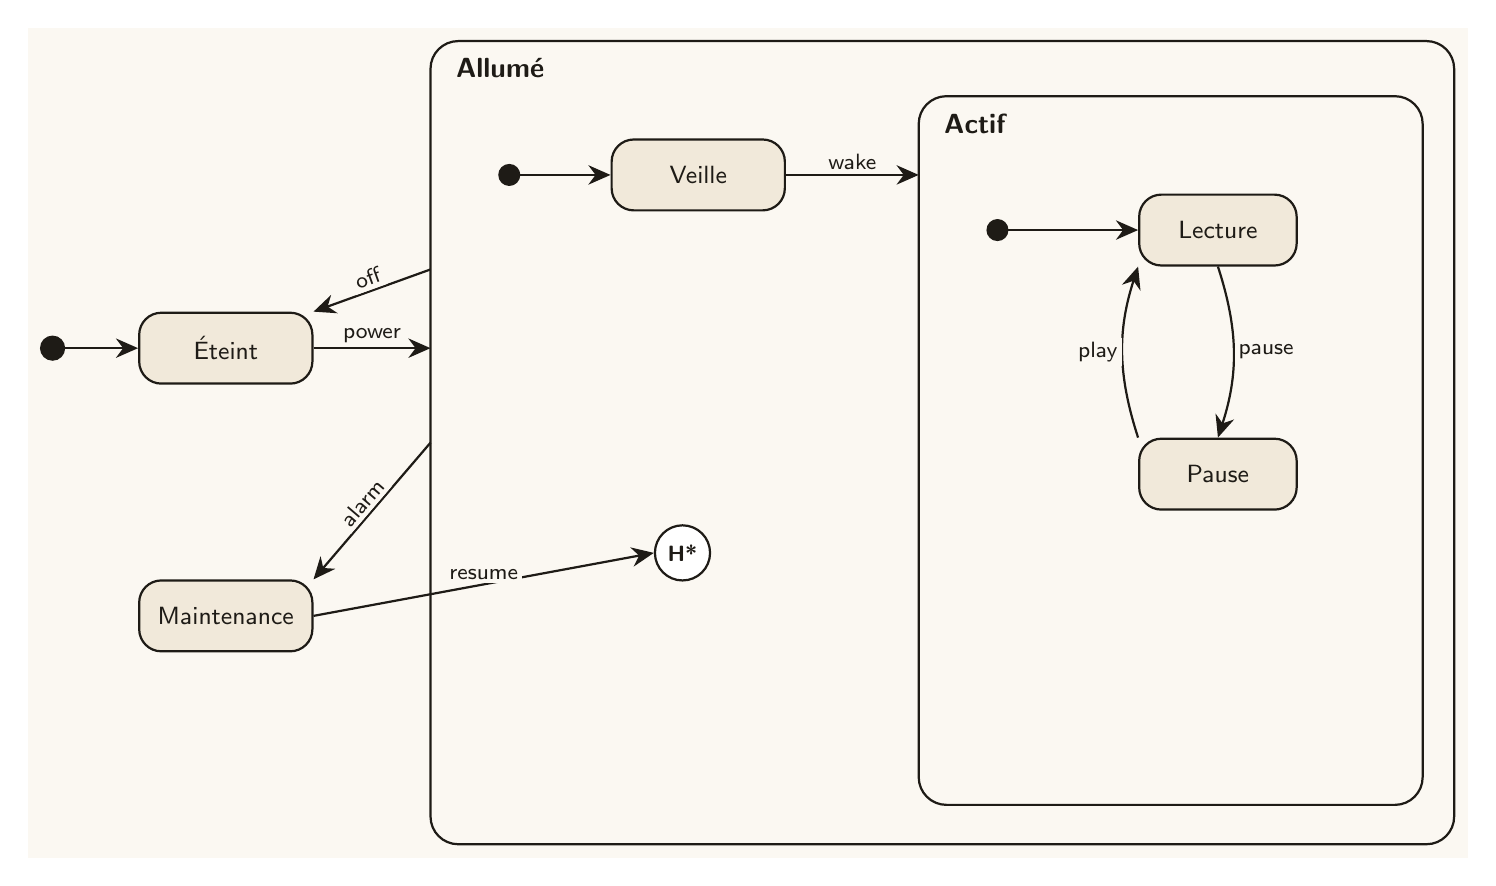
\begin{tikzpicture}[background rectangle/.style={fill=paper},show background rectangle]
\fill[ink] (-1.2,0) circle (0.16);
\node[state] (of) at (1.0,0) {Éteint};
\draw[line,-{Stealth[length=8pt,width=7pt]}] (-1.04,0)--(of.west);
\draw[line,rounded corners=10pt] (3.6,-6.3) rectangle (16.6,3.9);
\node[font=\bfseries,anchor=north west] at (3.8,3.8) {Allumé};
\fill[ink] (4.6,2.2) circle (0.14);
\node[state] (ve) at (7.0,2.2) {Veille};
\draw[line,-{Stealth[length=8pt,width=7pt]}] (4.74,2.2)--(ve.west);
\draw[line,rounded corners=10pt] (9.8,-5.8) rectangle (16.2,3.2);
\node[font=\bfseries,anchor=north west] at (10.0,3.1) {Actif};
\fill[ink] (10.8,1.5) circle (0.14);
\node[state,minimum width=2.0cm] (le) at (13.6,1.5) {Lecture};
\node[state,minimum width=2.0cm] (pa) at (13.6,-1.6) {Pause};
\draw[line,-{Stealth[length=8pt,width=7pt]}] (10.94,1.5)--(le.west);
\draw[line,-{Stealth[length=8pt,width=7pt]}] (le.south) to[bend left=18] node[right,lab]{pause} (pa.north);
\draw[line,-{Stealth[length=8pt,width=7pt]}] (pa.north west) to[bend left=18] node[left,lab]{play} (le.south west);
\draw[line,-{Stealth[length=8pt,width=7pt]}] (ve.east)--(9.8,2.2) node[midway,above,lab]{wake};
\node[circle,draw=ink,line width=0.8pt,fill=white,inner sep=1pt,minimum size=0.7cm,font=\footnotesize\bfseries] (h) at (6.8,-2.6) {H*};
\node[state] (ma) at (1.0,-3.4) {Maintenance};
\draw[line,-{Stealth[length=8pt,width=7pt]}] (of.east)--(3.6,0) node[midway,above,lab]{power};
\draw[line,-{Stealth[length=8pt,width=7pt]}] (3.6,-1.2)--(ma.north east) node[midway,above,sloped,lab]{alarm};
\draw[line,-{Stealth[length=8pt,width=7pt]}] (ma.east)--(h.west) node[midway,above,lab]{resume};
\draw[line,-{Stealth[length=8pt,width=7pt]}] (3.6,1.0)--(of.north east) node[midway,above,sloped,lab]{off};
\end{tikzpicture}
\end{document}
